\section{Auswertung und Diskussion}
\label{sec:DiskussionAuswertung}
In den Abbildungen \ref{fig:eoxmitptv}, \ref{fig:eoymitptv} und \ref{fig:eoz} sind die Dosisverteilungen des Schädels in der Transversal-, Sagittal- und Frontalansicht zu sehen. In den Abbildungen ist zu erkennen, dass die $\SI{95}{\percent}$ Isodosenlinie das rot eingezeichnete PTV vollständig umschließt. Für eine bessere Beurteilung ist das Dosis-Volumen-Histogramm in der Abbildung \ref{fig:dvheinzel} gezeigt.
Laut QUANTEC liegt der Dosisgrenzwert des Hirns bei einer maximalen Dosis von $\SI{60}{\gray}$. In der Bestrahlungsplanung ist es wichtig möglichst gut das Gehirn zu schonen und in diesem Fall beträgt die verordnete Dosis für die Bestrahlung bei $\SI{19,8}{\gray}$. Dabei ergibt sich kein Problem mit dem Dosisgrenzwert von QUANTEC. Das Dosismaximum des PTVs liegt bei $\SI{103.7}{\percent}$ von der $\SI{109}{\percent}$ maximal erlaubten Dosis. Das bedeutet, die vorgeschriebene maximal Dosis wird nicht überschritten und wurde dementsprechend eingehalten. Die minimale Dosis, die im PTV deponiert wird, liegt bei $\SI{87,7}{\percent}$. Das bedeutet, dass nicht das gesamte PTV mit einer relativen Dosis von $\SI{95}{\percent}$ bestrahlt wurde. Das kann anhand der Dosisverteilung erkannt werden. Nur ein geringer Teil des PTVs erhält eine relative Dosis von unter $\SI{95}{\percent}$, da in $\SI{99,3}{\percent}$ des PTV Volumens $\SI{95}{\percent}$ der Dosis deponiet wird. Anhand des DVHs (grüne Kurve) ist zu erkennen, dass der Hirn gut geschützt wird. Die mittlere Dosis des PTVs liegt hier bei $\SI{100}{\percent}$. Nur ein geringer Teil des PTVs (oben rechts) in der Darstellung \ref{fig:eoxmitptv} wird nicht von der $\SI{95}{\percent}$ Isodosenlinie umschlossen. Etwa $\SI{6}{\percent}$ des Volumens vom Hirn erhält noch eine relative Dosis von $\SI{50}{\percent}$. 
Die maximal Dosisbelastung für die Linsen liegt bei $\SI{5}{\gray}$. Die maximal Dosis der rechten Linse beträgt $\SI{3,75}{\gray}$ und der linken $\SI{2,175}{\gray}$. Fast $\SI{1}{\percent}$ von den Volumen der Linsen bekommen eine Dosis zwischen $\SI{0,9}{\gray}$ und $\SI{3,75}{\gray}$. Daraus folgt, dass die Linsen ausreichend geschont werden konnten. Das ist auch in der DVH (s. Abbildung \ref{fig:dvheinzel}) zu erkennen, weil die beiden Tiefendosiskurven relativ schnell abfallen.
Insgesamt lässt sich sagen, dass durch diesen Bestrahlungsplan mit zwei opponierenden Feldern die gewünschte Dosisverteilung im Hirn gut erreicht wird. 

\begin{figure}[htpb]
	\centering
	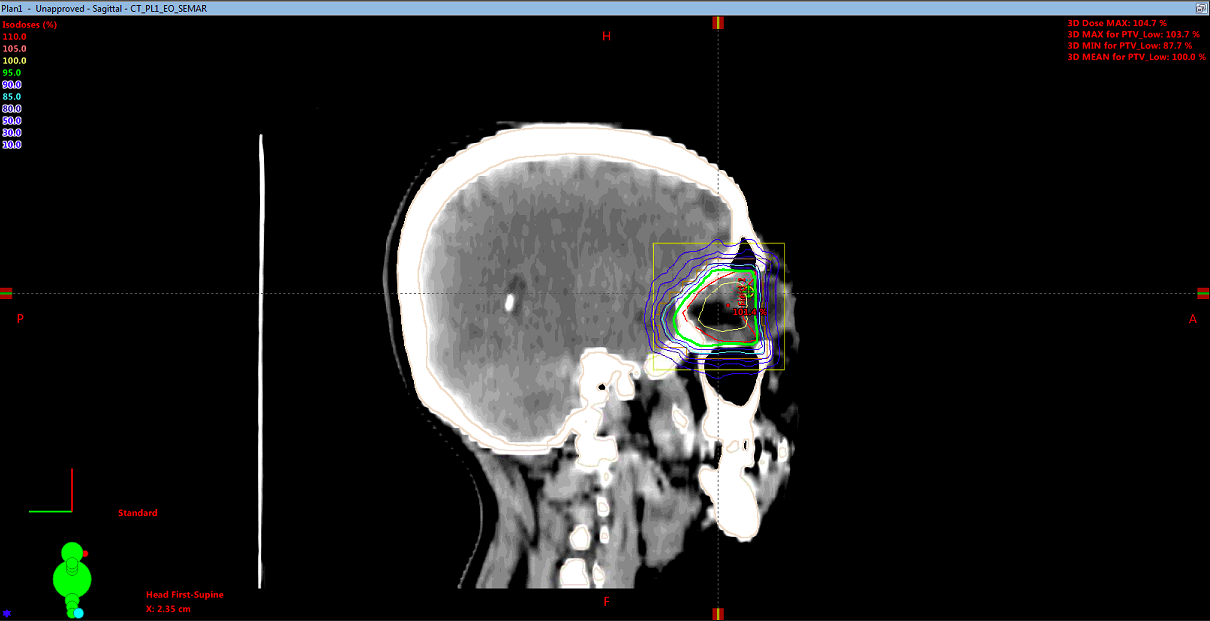
\includegraphics[width=0.7\linewidth]{../Bilder/EO_X_mitPTV}
	\caption{Darstellung der Dosisverteilung in der Sagittalansicht des Schädels.}
	\label{fig:eoxmitptv}
\end{figure}

\begin{figure}[htpb]
	\centering
	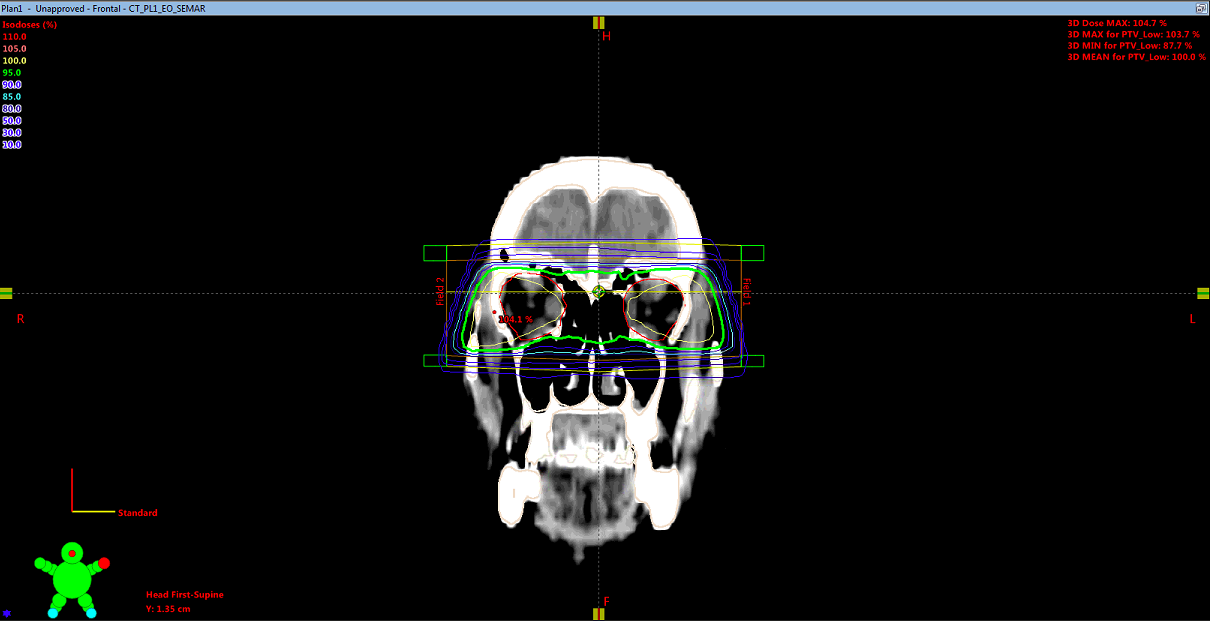
\includegraphics[width=0.7\linewidth]{../Bilder/EO_Y_mitPTV}
	\caption{Darstellung der Dosisverteilung in der Frontalansicht des Schädels.}
	\label{fig:eoymitptv}
\end{figure}

\begin{figure}[htpb]
	\centering
	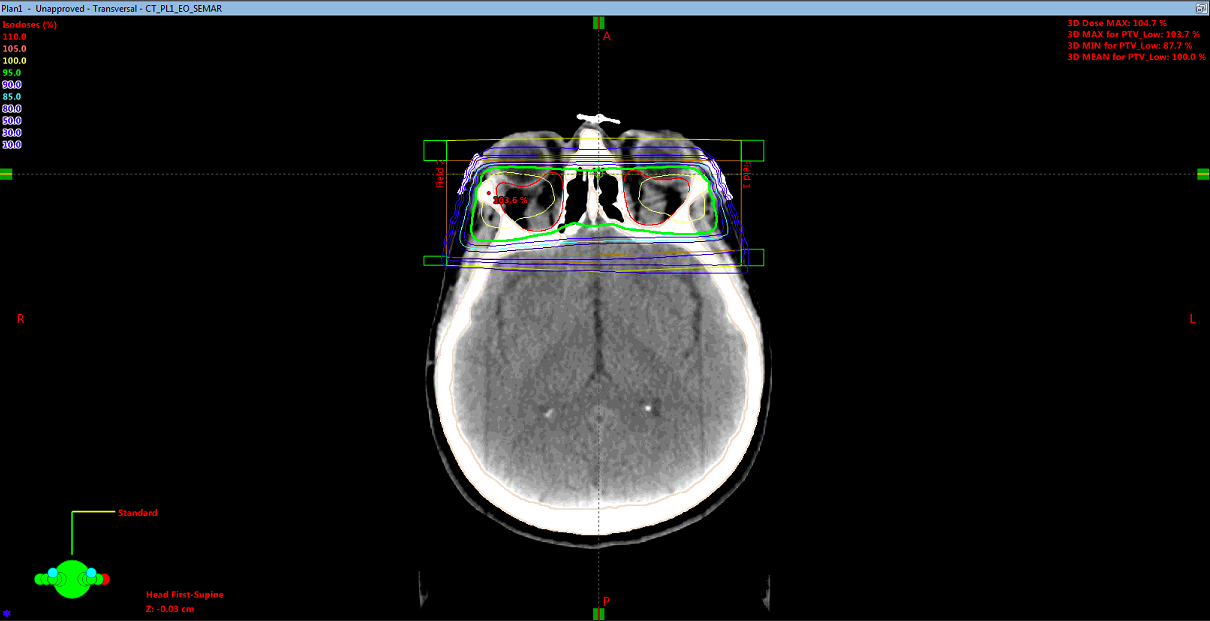
\includegraphics[width=0.7\linewidth]{../Bilder/EO_Z}
	\caption{Darstellung der Dosisverteilung in der Transversalansicht des Schädels.}
	\label{fig:eoz}
\end{figure}

\begin{figure}
	\centering
	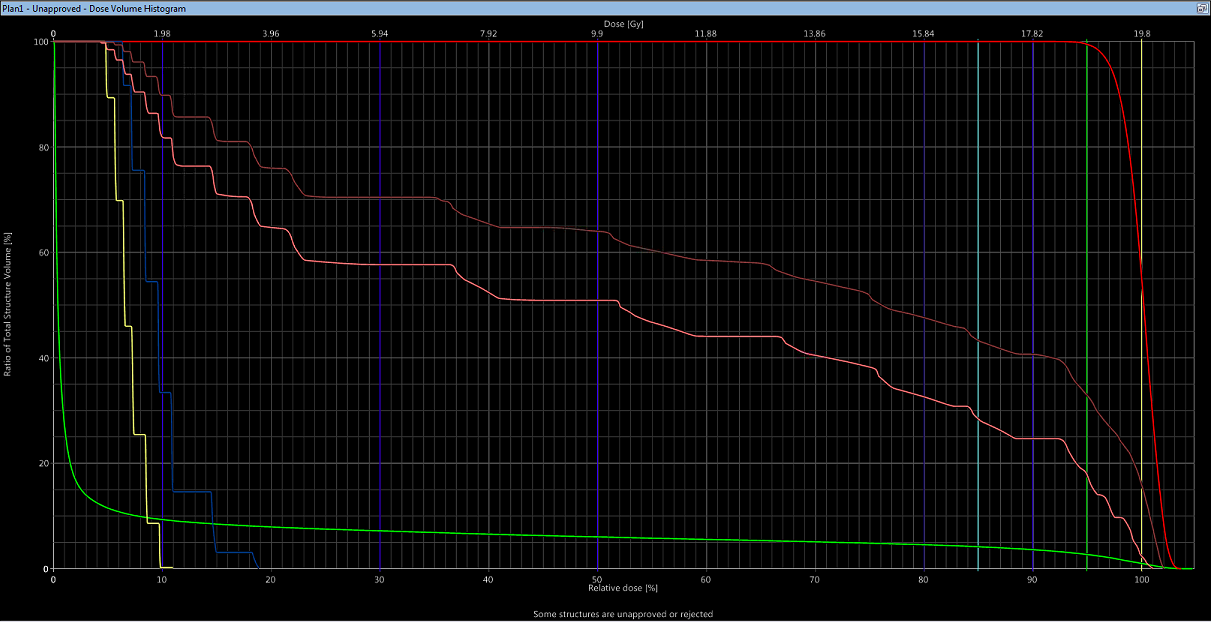
\includegraphics[width=0.7\linewidth]{../Bilder/DVH_Einzel}
	\caption{Zu sehen ist das DVH des Schädels. In roter Farbe dargestellt ist das PTV und in grüner Farbe ist der Schädel. Außerdem sind noch die einzelnen Isodosenlinien eingezeichnet und die einzelnen Kurven zu den Risikoorgane wie z.B. von den Linsen (gelb, dunkelblau) und Augen (pink,braun).}
	\label{fig:dvheinzel}
\end{figure}
